% this is a simplified version of 
% https://github.com/yihui/knitr/blob/master/inst/examples/knitr-beamer.Rnw
\documentclass{beamer}\usepackage[]{graphicx}\usepackage[]{color}
%% maxwidth is the original width if it is less than linewidth
%% otherwise use linewidth (to make sure the graphics do not exceed the margin)
\makeatletter
\def\maxwidth{ %
  \ifdim\Gin@nat@width>\linewidth
    \linewidth
  \else
    \Gin@nat@width
  \fi
}
\makeatother

\definecolor{fgcolor}{rgb}{0.345, 0.345, 0.345}
\newcommand{\hlnum}[1]{\textcolor[rgb]{0.686,0.059,0.569}{#1}}%
\newcommand{\hlstr}[1]{\textcolor[rgb]{0.192,0.494,0.8}{#1}}%
\newcommand{\hlcom}[1]{\textcolor[rgb]{0.678,0.584,0.686}{\textit{#1}}}%
\newcommand{\hlopt}[1]{\textcolor[rgb]{0,0,0}{#1}}%
\newcommand{\hlstd}[1]{\textcolor[rgb]{0.345,0.345,0.345}{#1}}%
\newcommand{\hlkwa}[1]{\textcolor[rgb]{0.161,0.373,0.58}{\textbf{#1}}}%
\newcommand{\hlkwb}[1]{\textcolor[rgb]{0.69,0.353,0.396}{#1}}%
\newcommand{\hlkwc}[1]{\textcolor[rgb]{0.333,0.667,0.333}{#1}}%
\newcommand{\hlkwd}[1]{\textcolor[rgb]{0.737,0.353,0.396}{\textbf{#1}}}%
\let\hlipl\hlkwb

\usepackage{framed}
\makeatletter
\newenvironment{kframe}{%
 \def\at@end@of@kframe{}%
 \ifinner\ifhmode%
  \def\at@end@of@kframe{\end{minipage}}%
  \begin{minipage}{\columnwidth}%
 \fi\fi%
 \def\FrameCommand##1{\hskip\@totalleftmargin \hskip-\fboxsep
 \colorbox{shadecolor}{##1}\hskip-\fboxsep
     % There is no \\@totalrightmargin, so:
     \hskip-\linewidth \hskip-\@totalleftmargin \hskip\columnwidth}%
 \MakeFramed {\advance\hsize-\width
   \@totalleftmargin\z@ \linewidth\hsize
   \@setminipage}}%
 {\par\unskip\endMakeFramed%
 \at@end@of@kframe}
\makeatother

\definecolor{shadecolor}{rgb}{.97, .97, .97}
\definecolor{messagecolor}{rgb}{0, 0, 0}
\definecolor{warningcolor}{rgb}{1, 0, 1}
\definecolor{errorcolor}{rgb}{1, 0, 0}
\newenvironment{knitrout}{}{} % an empty environment to be redefined in TeX

\usepackage{alltt}
\IfFileExists{upquote.sty}{\usepackage{upquote}}{}
\begin{document}

\title{Introducci\'on a la Gen\'omica \\ UNAL nov 2017}
\author{Alejandro C\'aceres \\ ISGlobal, Barcelona}


\maketitle
% very important to use option [fragile] for frames containing code output!


\begin{frame}[fragile]
\frametitle{Gen\'etica de poblaciones}

Los datos gen\'omicos de SNPs nos sirven para ver la variabilidad gen\'etica entre poblacines
\begin{itemize}
\item Estructura de LD en cada poblaci\'on
\item Heterocigosidad por poblaci\'on
\item \'Indice de fijaci\'on
\item Patrones de recombinaci\'on
\item Indicadores de selecci\'on
\item Filogenia
\end{itemize}
\end{frame}


\begin{frame}[fragile]
\frametitle{Estructura de LD entre poblaciones}

\begin{figure}[htbp]
\begin{center}
\includegraphics[width=.5\linewidth]{mozscreenshot141.pdf}
\end{center}
\end{figure}
\end{frame}


\begin{frame}[fragile]
\frametitle{C\'omo podemos extraer esa estructura}
\begin{table}[]
\centering
\begin{tabular}{c|cc|c}
  & A & T &  Total \\ \hline
C &  $x_{CA}$  &  $x_{CT}$  &  $q_C$ \\
A &  $x_{AA}$  &  $x_{AT}$  &  $q_A$  \\ \hline
Total & $p_A$  &  $p_T$  &   1 \\
\end{tabular}
\end{table}
el LD esta dado por $D=p_A*q_C - x_{CA}$

Recordemos que la fase se pierde por lo que el LD tiene que ser esimado modelando la probabilidad de una fase particular.

\end{frame}


\begin{frame}[fragile]
\frametitle{LD}
Con snpStats se puede calcular el LD entre dos SNPs

\begin{knitrout}\footnotesize
\definecolor{shadecolor}{rgb}{0.969, 0.969, 0.969}\color{fgcolor}\begin{kframe}
\begin{alltt}
\hlkwd{library}\hlstd{(snpStats)}
\end{alltt}
\end{kframe}
\end{knitrout}

\begin{knitrout}\footnotesize
\definecolor{shadecolor}{rgb}{0.969, 0.969, 0.969}\color{fgcolor}\begin{kframe}
\begin{alltt}
\hlkwd{load}\hlstd{(}\hlstr{"datos/NewsnpsSNPstats.RData"}\hlstd{)}
\hlkwd{ls}\hlstd{()}
\end{alltt}
\begin{verbatim}
## [1] "NewsnpsSNPstats"
\end{verbatim}
\end{kframe}
\end{knitrout}
\end{frame}


\begin{frame}[fragile]
\frametitle{LD}
Con snpStats se puede calcular el LD entre dos SNPs
\begin{knitrout}\footnotesize
\definecolor{shadecolor}{rgb}{0.969, 0.969, 0.969}\color{fgcolor}\begin{kframe}
\begin{alltt}
\hlstd{snps} \hlkwb{<-} \hlstd{NewsnpsSNPstats[,}\hlkwd{c}\hlstd{(}\hlnum{90}\hlstd{,}\hlnum{91}\hlstd{)]}
\hlkwd{ld}\hlstd{(snps,} \hlkwc{stats}\hlstd{=}\hlkwd{c}\hlstd{(}\hlstr{"D.prime"}\hlstd{,} \hlstr{"R.squared"}\hlstd{),}\hlkwc{depth}\hlstd{=}\hlnum{1}\hlstd{)}
\end{alltt}
\begin{verbatim}
## $D.prime
## 2 x 2 sparse Matrix of class "dgCMatrix"
##             rs561646592 rs34845889
## rs561646592           . 0.01220497
## rs34845889            . .         
## 
## $R.squared
## 2 x 2 sparse Matrix of class "dgCMatrix"
##             rs561646592   rs34845889
## rs561646592           . 8.640143e-05
## rs34845889            . .
\end{verbatim}
\end{kframe}
\end{knitrout}
\end{frame}

\begin{frame}[fragile]
\frametitle{LD}
Podemos tambi\'en calcular el LD entre todos los SNPs
\begin{knitrout}\footnotesize
\definecolor{shadecolor}{rgb}{0.969, 0.969, 0.969}\color{fgcolor}\begin{kframe}
\begin{alltt}
\hlstd{LD} \hlkwb{<-} \hlkwd{ld}\hlstd{(NewsnpsSNPstats,} \hlkwc{stats}\hlstd{=}\hlkwd{c}\hlstd{(}\hlstr{"D.prime"}\hlstd{,} \hlstr{"R.squared"}\hlstd{),}\hlkwc{depth}\hlstd{=}\hlnum{379}\hlstd{)}
\hlkwd{image}\hlstd{(LD}\hlopt{$}\hlstd{R.squared,} \hlkwc{lwd}\hlstd{=}\hlnum{0}\hlstd{)}
\end{alltt}
\end{kframe}
\includegraphics[width=.45\linewidth]{figure/plotLD-1} 

\end{knitrout}
\end{frame}



\begin{frame}[fragile]
\frametitle{LD}
LD para una poblaci\'on

Seleccionemos los individuos de la poblaci\'on GBR

\begin{knitrout}\footnotesize
\definecolor{shadecolor}{rgb}{0.969, 0.969, 0.969}\color{fgcolor}\begin{kframe}
\begin{alltt}
\hlstd{ids} \hlkwb{<-} \hlkwd{read.table}\hlstd{(}\hlstr{"datos/20130606_g1k.ped"}\hlstd{,} \hlkwc{sep}\hlstd{=}\hlstr{"\textbackslash{}t"}\hlstd{,} \hlkwc{header}\hlstd{=}\hlnum{TRUE}\hlstd{)}

\hlkwd{rownames}\hlstd{(ids)} \hlkwb{<-} \hlstd{ids}\hlopt{$}\hlstd{Individual.ID}
\hlstd{pops} \hlkwb{<-} \hlstd{ids[}\hlkwd{rownames}\hlstd{(NewsnpsSNPstats),]}\hlopt{$}\hlstd{Population}
\hlkwd{head}\hlstd{(pops)}
\end{alltt}
\begin{verbatim}
## [1] GBR GBR GBR GBR GBR GBR
## 26 Levels: ACB ASW BEB CDX CEU CHB CHS CLM ESN FIN GBR GIH GWD IBS ... YRI
\end{verbatim}
\begin{alltt}
\hlstd{GBR} \hlkwb{<-} \hlstd{pops}\hlopt{==}\hlstr{"GBR"}
\hlkwd{head}\hlstd{(GBR)}
\end{alltt}
\begin{verbatim}
## [1] TRUE TRUE TRUE TRUE TRUE TRUE
\end{verbatim}
\end{kframe}
\end{knitrout}
\end{frame}

\begin{frame}[fragile]
\frametitle{LD}
LD para GRB

\begin{knitrout}\footnotesize
\definecolor{shadecolor}{rgb}{0.969, 0.969, 0.969}\color{fgcolor}\begin{kframe}
\begin{alltt}
\hlstd{snpsGBR} \hlkwb{<-} \hlstd{NewsnpsSNPstats[GBR,]}
\hlstd{LDGBR} \hlkwb{<-} \hlkwd{ld}\hlstd{(snpsGBR,} \hlkwc{stats}\hlstd{=}\hlkwd{c}\hlstd{(}\hlstr{"D.prime"}\hlstd{,} \hlstr{"R.squared"}\hlstd{),}\hlkwc{depth}\hlstd{=}\hlnum{379}\hlstd{)}
\hlkwd{image}\hlstd{(LDGBR}\hlopt{$}\hlstd{R.squared,} \hlkwc{lwd}\hlstd{=}\hlnum{0}\hlstd{)}
\end{alltt}
\end{kframe}
\includegraphics[width=.45\linewidth]{figure/plotLDGRB-1} 

\end{knitrout}
\end{frame}

\begin{frame}[fragile]
\frametitle{LD}
Ejercicio LD para una poblaci\'on YRI

\begin{knitrout}\footnotesize
\definecolor{shadecolor}{rgb}{0.969, 0.969, 0.969}\color{fgcolor}
\includegraphics[width=.45\linewidth]{figure/plotLDYRI-1} 
\includegraphics[width=.45\linewidth]{figure/plotLDYRI-2} 

\end{knitrout}
\end{frame}

\begin{frame}[fragile]
\frametitle{LD}
Ejercicio LD para una poblaci\'on YRI

\begin{knitrout}\footnotesize
\definecolor{shadecolor}{rgb}{0.969, 0.969, 0.969}\color{fgcolor}\begin{kframe}
\begin{alltt}
\hlstd{YRI} \hlkwb{<-} \hlstd{pops}\hlopt{==}\hlstr{"YRI"}
\hlstd{snpsYRI} \hlkwb{<-} \hlstd{NewsnpsSNPstats[YRI,]}
\hlstd{LDYRI} \hlkwb{<-} \hlkwd{ld}\hlstd{(snpsYRI,} \hlkwc{stats}\hlstd{=}\hlkwd{c}\hlstd{(}\hlstr{"D.prime"}\hlstd{,} \hlstr{"R.squared"}\hlstd{),}\hlkwc{depth}\hlstd{=}\hlnum{379}\hlstd{)}
\hlkwd{image}\hlstd{(LDYRI}\hlopt{$}\hlstd{R.squared,} \hlkwc{lwd}\hlstd{=}\hlnum{0}\hlstd{)}
\end{alltt}
\end{kframe}
\end{knitrout}
\end{frame}




\begin{frame}[fragile]
\frametitle{Heterecigosidad}
\begin{itemize}
\item La heterocigosidad es la proporci\'on de heterocigotos que hay en una poblaci\'on.
\item Mayor taza de heterocigosidad mayor es la variabilidad gen\'etica
\end{itemize}
se calcula como 
\begin{eqnarray}
2pq=1-p^2-q^2
\end{eqnarray}

\end{frame}

\begin{frame}[fragile]
\frametitle{Heterecigosidad}

\begin{knitrout}\footnotesize
\definecolor{shadecolor}{rgb}{0.969, 0.969, 0.969}\color{fgcolor}\begin{kframe}
\begin{alltt}
\hlstd{sumSnps} \hlkwb{<-} \hlkwd{col.summary}\hlstd{(NewsnpsSNPstats)}
\hlkwd{head}\hlstd{(sumSnps)}
\end{alltt}
\begin{verbatim}
##             Calls Call.rate Certain.calls        RAF        MAF      P.AA
## rs555347111  2504         1             1 0.07368211 0.07368211 0.8554313
## rs542617372  2504         1             1 0.07607827 0.07607827 0.8582268
## rs17763596   2504         1             1 0.07767572 0.07767572 0.8586262
## rs144873025  2504         1             1 0.08047125 0.08047125 0.8486422
## rs184461291  2504         1             1 0.07607827 0.07607827 0.8514377
## rs566494525  2504         1             1 0.06709265 0.06709265 0.8674121
##                  P.AB        P.BB     z.HWE
## rs555347111 0.1417732 0.002795527  1.930779
## rs542617372 0.1313898 0.010383387 -3.271542
## rs17763596  0.1273962 0.013977636 -5.548735
## rs144873025 0.1417732 0.009584665 -2.102509
## rs184461291 0.1449681 0.003594249  1.561671
## rs566494525 0.1309904 0.001597444  2.321653
\end{verbatim}
\end{kframe}
\end{knitrout}
\end{frame}



\begin{frame}[fragile]
\frametitle{Heterecigosidad}

\begin{knitrout}\footnotesize
\definecolor{shadecolor}{rgb}{0.969, 0.969, 0.969}\color{fgcolor}\begin{kframe}
\begin{alltt}
\hlstd{p}\hlkwb{<-}\hlstd{sumSnps}\hlopt{$}\hlstd{MAF}
\hlkwd{hist}\hlstd{(}\hlnum{1}\hlopt{-}\hlstd{p}\hlopt{^}\hlnum{2}\hlopt{-}\hlstd{(}\hlnum{1}\hlopt{-}\hlstd{p)}\hlopt{^}\hlnum{2}\hlstd{)}
\end{alltt}
\end{kframe}
\includegraphics[width=.45\linewidth]{figure/unnamed-chunk-7-1} 

\end{knitrout}
\end{frame}


\begin{frame}[fragile]
\frametitle{Heterecigosidad}
Heterocigosidad en una poblaci\'on

\begin{knitrout}\footnotesize
\definecolor{shadecolor}{rgb}{0.969, 0.969, 0.969}\color{fgcolor}\begin{kframe}
\begin{alltt}
\hlstd{lv} \hlkwb{<-} \hlkwd{levels}\hlstd{(pops)}
\hlstd{x} \hlkwb{<-} \hlstd{lv[}\hlnum{1}\hlstd{]}
\hlstd{x}
\end{alltt}
\begin{verbatim}
## [1] "ACB"
\end{verbatim}
\begin{alltt}
\hlstd{whichpop} \hlkwb{<-} \hlstd{pops}\hlopt{==}\hlstd{x}
\hlstd{POPsnps} \hlkwb{<-} \hlstd{NewsnpsSNPstats[whichpop,]}
\hlstd{sumSnps} \hlkwb{<-} \hlkwd{col.summary}\hlstd{(POPsnps)}
\hlstd{p} \hlkwb{<-} \hlstd{sumSnps}\hlopt{$}\hlstd{MAF}
\end{alltt}
\end{kframe}
\end{knitrout}
\end{frame}

\begin{frame}[fragile]
\frametitle{Heterecigosidad}
Heterocigosidad en una poblaci\'on

\begin{knitrout}\footnotesize
\definecolor{shadecolor}{rgb}{0.969, 0.969, 0.969}\color{fgcolor}\begin{kframe}
\begin{alltt}
\hlkwd{hist}\hlstd{(}\hlnum{1}\hlopt{-}\hlstd{p}\hlopt{^}\hlnum{2}\hlopt{-}\hlstd{(}\hlnum{1}\hlopt{-}\hlstd{p)}\hlopt{^}\hlnum{2}\hlstd{)}
\end{alltt}
\end{kframe}
\includegraphics[width=.45\linewidth]{figure/unnamed-chunk-9-1} 

\end{knitrout}

\end{frame}

\begin{frame}[fragile]
\frametitle{LD}
Histograma de heterocigosidad para YRI
\begin{knitrout}\footnotesize
\definecolor{shadecolor}{rgb}{0.969, 0.969, 0.969}\color{fgcolor}\begin{kframe}
\begin{verbatim}
## [1] "YRI"
\end{verbatim}
\end{kframe}
\includegraphics[width=.45\linewidth]{figure/unnamed-chunk-10-1} 

\end{knitrout}
\end{frame}


\begin{frame}[fragile]
\frametitle{LD}
Histograma de heterocigosidad para YRI
\begin{knitrout}\footnotesize
\definecolor{shadecolor}{rgb}{0.969, 0.969, 0.969}\color{fgcolor}\begin{kframe}
\begin{alltt}
\hlstd{lv} \hlkwb{<-} \hlkwd{levels}\hlstd{(pops)}
\hlstd{x} \hlkwb{<-} \hlstd{lv[}\hlnum{26}\hlstd{]}
\hlstd{x}
\hlstd{whichpop} \hlkwb{<-} \hlstd{pops}\hlopt{==}\hlstd{x}
\hlstd{POPsnps} \hlkwb{<-} \hlstd{NewsnpsSNPstats[whichpop,]}
\hlstd{sumSnps} \hlkwb{<-} \hlkwd{col.summary}\hlstd{(POPsnps)}
\hlstd{p} \hlkwb{<-} \hlstd{sumSnps}\hlopt{$}\hlstd{MAF}
\hlkwd{hist}\hlstd{(}\hlnum{1}\hlopt{-}\hlstd{p}\hlopt{^}\hlnum{2}\hlopt{-}\hlstd{(}\hlnum{1}\hlopt{-}\hlstd{p)}\hlopt{^}\hlnum{2}\hlstd{)}
\end{alltt}
\end{kframe}
\end{knitrout}

\end{frame}




\begin{frame}[fragile]
\frametitle{Heterecigosidad}
Heterocigosidad por poblaciones

\begin{knitrout}\footnotesize
\definecolor{shadecolor}{rgb}{0.969, 0.969, 0.969}\color{fgcolor}\begin{kframe}
\begin{alltt}
\hlstd{hetpop}\hlkwb{<-}\hlkwd{sapply}\hlstd{(}\hlkwd{levels}\hlstd{(pops),} \hlkwa{function}\hlstd{(}\hlkwc{x}\hlstd{)}
 \hlstd{\{}
    \hlstd{whichpop} \hlkwb{<-} \hlstd{pops}\hlopt{==}\hlstd{x}
    \hlstd{POPsnps} \hlkwb{<-} \hlstd{NewsnpsSNPstats[whichpop,]}
    \hlstd{sumSnps} \hlkwb{<-} \hlkwd{col.summary}\hlstd{(POPsnps)}
    \hlstd{p} \hlkwb{<-} \hlstd{sumSnps}\hlopt{$}\hlstd{MAF}
    \hlnum{1}\hlopt{-}\hlstd{p}\hlopt{^}\hlnum{2}\hlopt{-}\hlstd{(}\hlnum{1}\hlopt{-}\hlstd{p)}\hlopt{^}\hlnum{2}
  \hlstd{\})}
\hlstd{hetpop[}\hlnum{1}\hlopt{:}\hlnum{5}\hlstd{,}\hlnum{1}\hlopt{:}\hlnum{5}\hlstd{]}
\end{alltt}
\begin{verbatim}
##            ACB        ASW       BEB        CDX       CEU
## [1,] 0.1948242 0.01625907 0.1965251 0.16608857 0.1569738
## [2,] 0.1440430 0.12254770 0.2401298 0.07243612 0.1735027
## [3,] 0.2341580 0.07860790 0.2230936 0.20857903 0.1226916
## [4,] 0.1614041 0.15049718 0.1592077 0.16608857 0.2130395
## [5,] 0.1614041 0.10816985 0.2230936 0.13920684 0.1816141
\end{verbatim}
\end{kframe}
\end{knitrout}
\end{frame}


\begin{frame}[fragile]
\frametitle{Heterecigosidad}
Heterocigosidad por poblaciones

\begin{knitrout}\footnotesize
\definecolor{shadecolor}{rgb}{0.969, 0.969, 0.969}\color{fgcolor}\begin{kframe}
\begin{alltt}
\hlkwd{boxplot}\hlstd{(hetpop)}
\end{alltt}
\end{kframe}
\includegraphics[width=.45\linewidth]{figure/unnamed-chunk-13-1} 

\end{knitrout}
\end{frame}



\begin{frame}[fragile]
\frametitle{\'Indice de fijaci\'on}

El Fst (fixation index) que mide la proporcion de variabilidad genetica debida a diferencias entre poblaciones 
\begin{eqnarray}
F_{ST}=\frac{\sigma^2_S}{\sigma^2_T}
\end{eqnarray}

$\sigma^2_S$ es la varianza entre poblaciones y $\sigma^2_T$ es la varianza total
\end{frame}

\begin{frame}[fragile]
\frametitle{\'Indice de fijaci\'on}

\begin{figure}[htbp]
\begin{center}
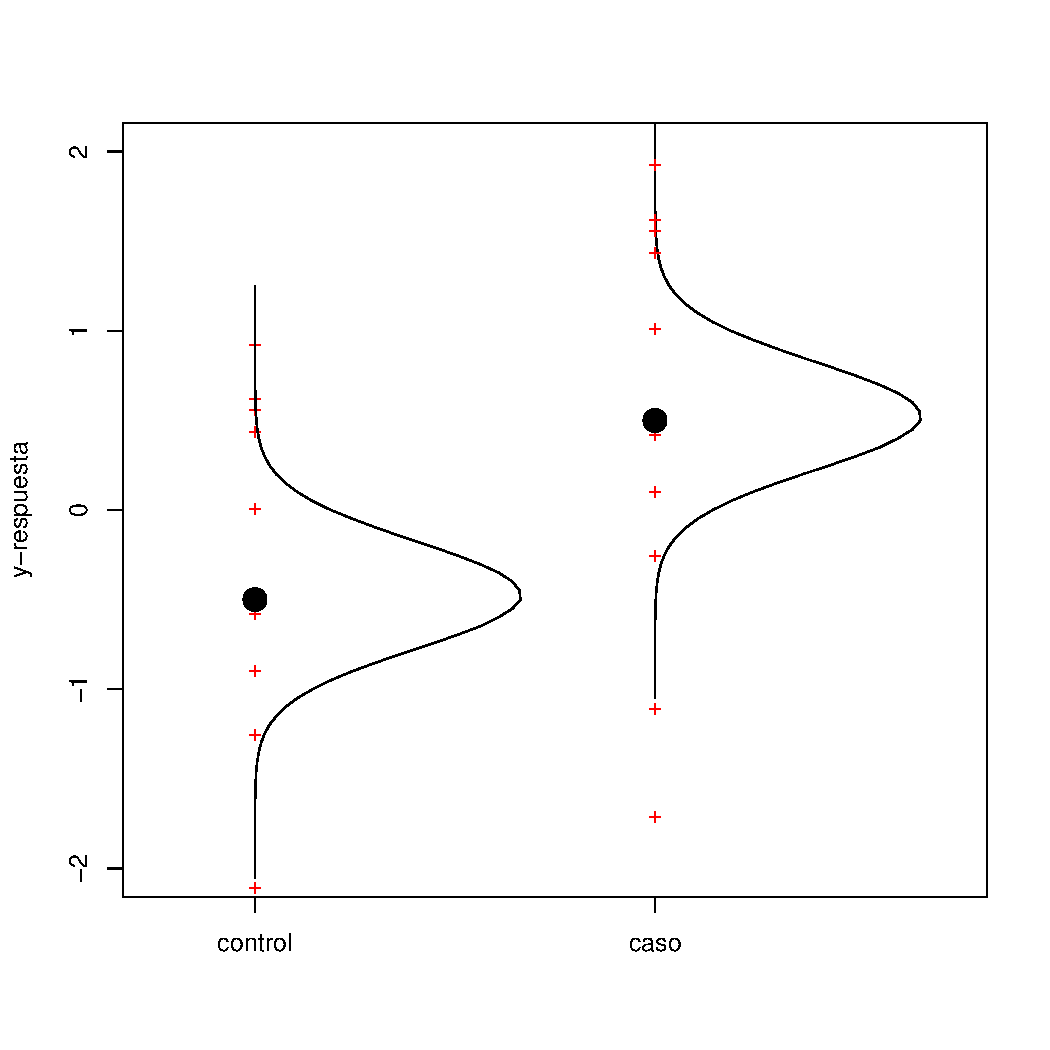
\includegraphics[width=.5\linewidth]{twogroup.pdf}
\end{center}
\end{figure}

\begin{eqnarray}
F=\frac{\sigma^2_{caso-control}}{\sigma^2_{todos}}
\end{eqnarray}
Qu\'e tan differenciables son los groupos?

\end{frame}

\begin{frame}[fragile]
Distribuci\'on de Fst en la regi\'on de \emph{MAPT} para los 1000 genomas 
\frametitle{Fst}
\begin{knitrout}\footnotesize
\definecolor{shadecolor}{rgb}{0.969, 0.969, 0.969}\color{fgcolor}\begin{kframe}
\begin{alltt}
\hlstd{FST} \hlkwb{<-} \hlkwd{Fst}\hlstd{(NewsnpsSNPstats,pops)}
\hlkwd{hist}\hlstd{(FST}\hlopt{$}\hlstd{Fst)}
\end{alltt}
\end{kframe}
\includegraphics[width=.45\linewidth]{figure/plotfst-1} 

\end{knitrout}
\end{frame}


\begin{frame}[fragile]
Fst promedio estimado para las poblaciones del HapMap 

\begin{table}[]
\frametitle{Fst}
\centering
\begin{tabular}{c|ccc}
 	&CEU&	YRI &	JPT \\ \hline
YRI &	0.153 \\ 		
JPT&	0.111 &	0.190 \\	
CHB &	0.110 &	0.192 &	0.007 \\
\end{tabular}
\end{table}
\end{frame}

\begin{frame}[fragile]
\frametitle{Fst}

Ejercicio: calcular Fst entre YRI y CEU en la region de \emph{MAPT}

\begin{knitrout}\footnotesize
\definecolor{shadecolor}{rgb}{0.969, 0.969, 0.969}\color{fgcolor}\begin{kframe}
\begin{verbatim}
## [1] 0.003333865
\end{verbatim}
\end{kframe}
\includegraphics[width=.45\linewidth]{figure/unnamed-chunk-14-1} 

\end{knitrout}
\end{frame}


\begin{frame}[fragile]
\frametitle{Fst}

Ejercicio: calcular Fst entre YRI y CEU en la region de \emph{MAPT}

\begin{knitrout}\footnotesize
\definecolor{shadecolor}{rgb}{0.969, 0.969, 0.969}\color{fgcolor}\begin{kframe}
\begin{alltt}
\hlstd{CEUandYRI} \hlkwb{<-} \hlstd{pops}\hlopt\hlkwd{c}\hlstd{(}\hlstr{"CEU"}\hlstd{,}\hlstr{"YRI"}\hlstd{)}
\hlstd{snpsCEUandYRI}\hlkwb{<-}\hlstd{NewsnpsSNPstats[CEUandYRI,]}
\hlstd{popsCEUandYRI} \hlkwb{<-} \hlstd{pops[CEUandYRI]}
\hlstd{FST} \hlkwb{<-} \hlkwd{Fst}\hlstd{(snpsCEUandYRI,popsCEUandYRI)}
\hlkwd{hist}\hlstd{(FST}\hlopt{$}\hlstd{Fst)}
\hlkwd{mean}\hlstd{(FST}\hlopt{$}\hlstd{Fst,} \hlkwc{na.rm}\hlstd{=}\hlnum{TRUE}\hlstd{)}
\end{alltt}
\end{kframe}
\end{knitrout}
\end{frame}

\begin{frame}[fragile]
\frametitle{Fst y heterocigosidad en 1000 Genomas}

Livio Casarini  et al. Clin Endocrinol Metab, 2014, 99(11):E2412

\begin{figure}[htbp]
\begin{center}
\includegraphics[width=1\linewidth]{1000gFst.png}
\end{center}
\end{figure}
\end{frame}


\end{document}
